\chapter{Fundamentos te\'oricos}\label{capit:cap2}
\vspace{-2.0325ex}%
\noindent
\rule{\textwidth}{0.5pt}
\vspace{-5.5ex}% 
\newcommand{\pushline}{\Indp}% Indent puede ir o no :p

\section{Introducci\'on}\label{secc:introduccion}





\section{Qu\'e es la Ansiedad?}\label{secc:ansiedad}

La ansiedad es una emoci\'on caracterizada por sensaciones de tensi\'on, pensamientos de preocupaci\'on y cambios f\'isicos como incremento en la presi\'on arterial \citep{psychologyapa}, aumento de la sudoraci\'on y palpitaciones, entre otras respuestas fisiol\'ogicas. Estas manifestaciones se dan en determinados lapsos de tiempos durante la vida del individuo. Durante estos lapsos, se dice que el sujeto se encuentra en un estado mental de ansiedad [ref].

Este estado mental es \'util para los humanos, debido a que la ansiedad es una reacci\'on normal del cuerpo para lograr objetivos, o lograr sobrevivir ante a una amenaza. Sin embargo, cuando la persona experimenta un nivel de ansiedad el cual es tan alto que no le permite manejar su vida normal, se dice que la persona tiene un desorden de ansiedad\citep{repetto2013}. 


\subsection{``State Anxiety'' y ``Trait Anxiety''}\label{secc:anxieystatevstrait}
Existen dos clasificaciones de ansiedad definidas por la psicolog\'ia[ref], ``State Anxiety'' y ``Trait Anxiety'' las cuales se mencionan a continuaci\'on.

\begin{itemize}
	\item{\textbf{State Anxiety:}} Es una manifestaci\'on de ansiedad a cerca de un evento \textbf{presente} bien definido. Normalmente la persona se encuentra conciente de la fuente de su ansiead. 
	\item{\textbf{Trait Anxiety:}} Es una manifestaci\'on a largo plazo de la ansiedad, en la que el individuo puede entrar al estado de ansiedad sin saber la raz\'on concreta. Las personas con personalidades t\'imidas tienden a sufrir mas de este tipo de ansiedad. [ref]

\end{itemize}

A pesar de que los efectos negativos en la calidad de vida de las personas que sufren de ``Trait Anxiety'' son mas fuertes, este trabajo est\'a enfocado en ``State Anxiety'' debido a que es mas f\'acil de cuantificar y medir por medio de sensores.

\subsection{Ansiedad y estr\'es}\label{secc:anxietyandstress}
%Una forma com\'un en donde la ansiedad se presenta es en el estr\'es. La relaci\'on entre el estr\'es y la ansiedad es la ansiedad es la se\~nal psicofisiol\'ogica de que la respuesta al estr\'es ha sido iniciada \citep{PMID2235645}. Es com\'un que la poblaci\'on en general tenga episodios de ansiedad debido a los tipos de trabajo de nuestra sociedad moderna. 
Si bien, en ocasiones el estr\'es y la ansiedad son conceptos que se usan de manera intercambiable, existen diferencias entre ambos. El estr\'es es definido como el desvalance entre la carga mental dada y la percepci\'on de las habilidades que el individuo tiene para lidiar dicha carga[ref]. Este desvalance puede hacer que la ansiedad aumente, mientras que la ansiedad puede a su vez generar estr\'es.

\section{Demencia}\label{secc:dementia}
La demencia es un s\'indrome del declive de las habilidades cognitivas. Los s\'intomas comunes son: problemas de memoria, dificultades para realizar tareas familiares, mal juicio, deterioro del lenguaje hablado y cambios de humor\citep{Aziz}. Afecta alrededor de el 4\% de las personas mayores de 65 a\~nos y al 40\% de las personas mayores de 90. La demencia suele manifestarse en sindromes como el de Alzheimer. Las personas con demencia necesitan de una persona que cuide de ellos, normalmente durante el resto de su vida. Usualmente necesitan ayuda en las actividades de la vida diaria (Activities of Daily Life), siendo esto una carga para los cuidadores.

\section{Cuidadores}\label{secc:caregivers}
Uno de los sectores de poblaci\'on vulnerables, son los cuidadores de personas con demencia. Se encuentra documentado que los cuidadores, al llevar una carga f\'isica, cognitiva y emocional derivada de su labor les genera padecimientos como ansiedad, estr\'es, y hasta la muerte\citep{Chen2013}. Debido a que los cuidadores no necesariamente son personas con una formaci\'on profesional, estos efectos pueden verse aumentados. Por lo general, los cuidadores que son familiares del paciente son a\'un m\'as afectados ya que necesitan administrar el tiempo de trabajo, familia, actividades sociales y la actividad misma del cuidado del paciente.
			%Cuales son las situaciones ( escenarios ) en los que los CUIDADORES presentan ansiedad?

\subsection{C\'omo se genera la ansiedad en los cuidadores?}\label{secc:caregiverburden}

\begin{figure}[h]
	\centering
	\subfigure[]{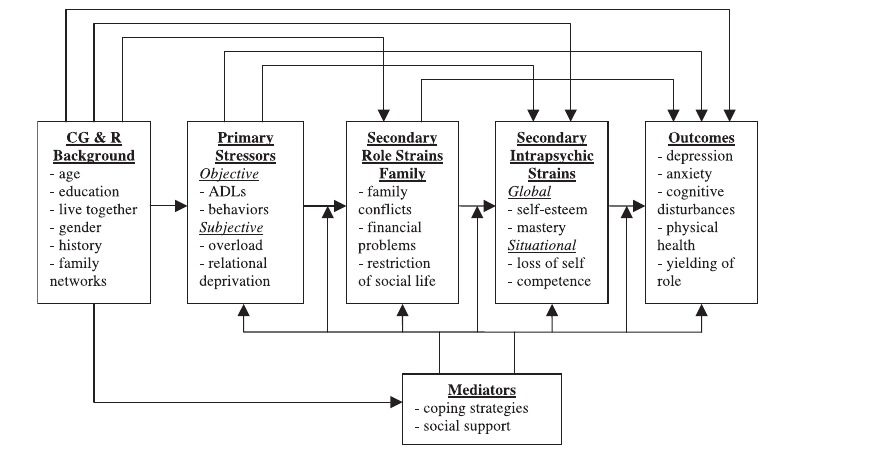
\includegraphics[width=160mm,height=80mm]{./Figures/img_frame}} 
	\caption{El modelo de ansiedad en cuidadores [ref] (Pearlin et al 1990)} \label{fig:instauracionFatigaReposo}
\end{figure}

\subsection{Cuidadores Formales e Informales}\label{secc:caregivers}
\section{C\'omputo vestible}\label{secc:dementia}
El c\'omputo vestible nos permite llevar computadoras con nosotros de la misma manera que llevamos la ropa puesta. Al ``vestir'' un dispositivo, el usuario tiene acceso a una computadora que es capaz de monitorearlo a \'el y a su entorno por medio de sensores. Los sensores pueden medir entre otras cosas: movimientos del cuerpo del usuario, la posici\'on del usuario, intensidad de luz, ruido, im\'agenes de su ambiente, ritmo card\'iaco, capacidad conductiva de la piel, distancias, actividad cerebral, entre otros. Debido a la cercania con el usuario, se pueden hacer monitoreos constantes y mas precisos que con los sistemas tradicionales y ayudar en las tareas de la vida cotidiana.

El uso de c\'omputo vestible abre la posibilidad de detectar la ansiedad por medio de las se\~nales fisiol\'ogicas del usuario.

\section{Trabajo previo en detecci\'on de ansiedad}

*Trabajos de Bert
*
\section{Conclusion}\label{secc:conclution}



\newpage
%%=====================================================
